\section{Introduction}

Frontier-based navigation agents~\cite{11168188} score candidate frontiers with a function that is fixed for the entire episode. A frontier encountered late in a trajectory is assessed with the same model, confidence, and explore-exploit balance as one encountered at the start. In Embodied Question Answering (EQA)~\cite{jiang2025beyond}, where an agent must navigate an unfamiliar 3D environment to gather evidence for a natural-language question, this rigidity is costly, since the agent must decide what to search for and how long to keep looking with no way to hold its own mistakes against its next decision.

Recent memory-augmented EQA methods~\cite{huang20243dmem,wang2026memoryexplorer,zhang2026fast} show that richer memory yields better answers, but they inherit whatever observations navigation provides, and no retrieval mechanism can recover evidence the agent never collected. Progress on memory has outpaced progress on the search that feeds it.

\begin{figure*}[t]
\centering
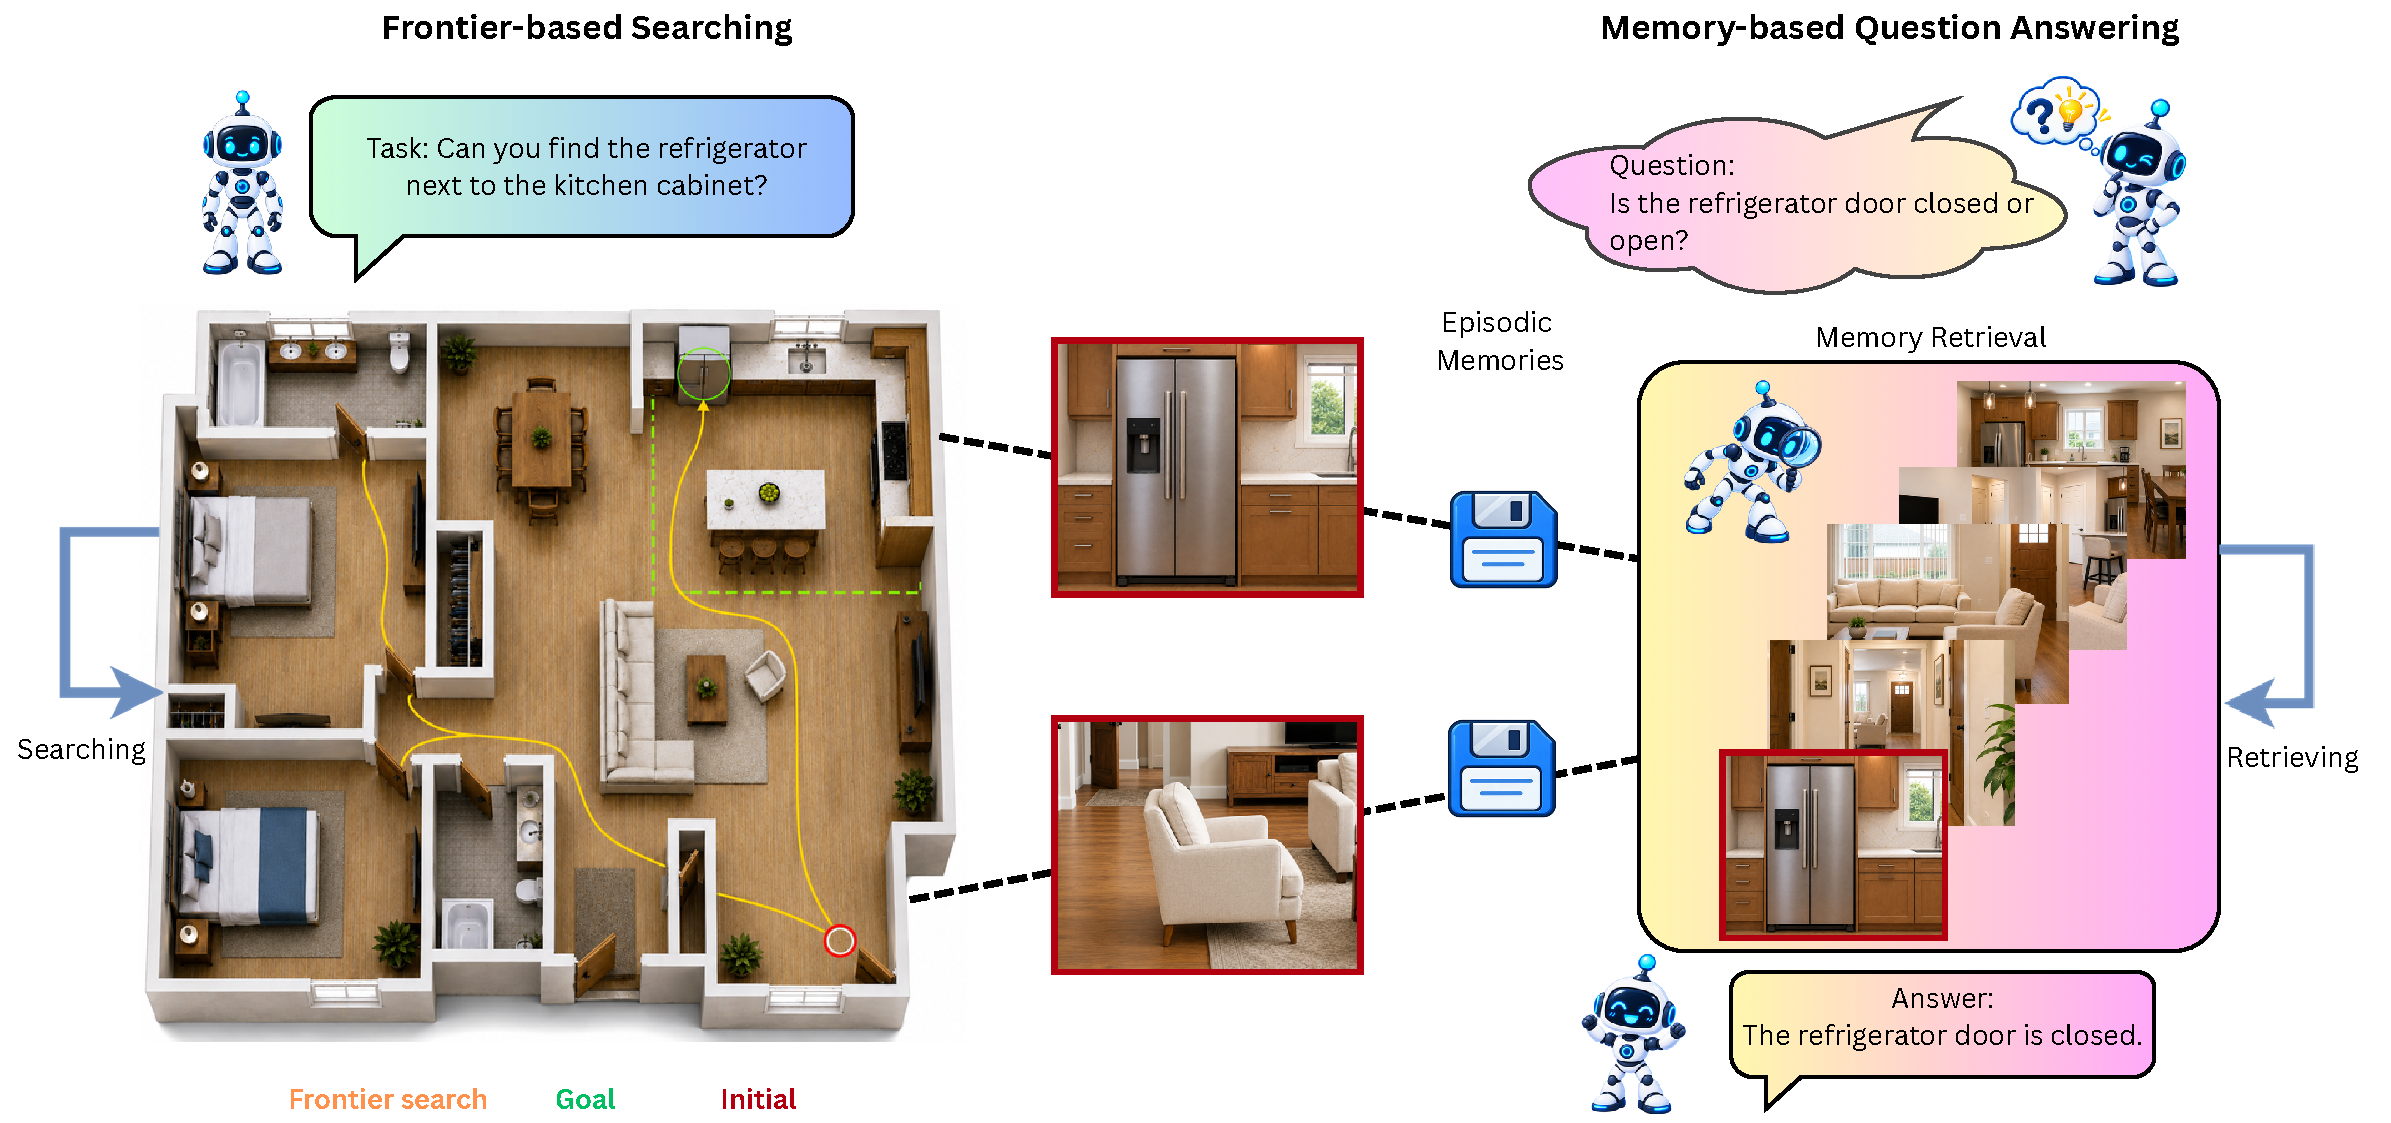
\includegraphics[width=0.92\textwidth]{figures/teaser.pdf}
\caption{\textbf{The EQA problem.} An agent must search an unseen environment by frontier exploration to reach a described target, storing observations as episodic memory, and later answer follow-up questions by retrieving from that memory. What the search fails to observe, retrieval cannot recover.}
\label{fig:teaser}
\end{figure*}

A second opportunity lies in how the task is posed. Long-horizon benchmarks treat every object named in an instruction as a terminal goal. We read them differently. An instruction names its target inside relational context, the rooms it sits in and the objects beside it, and that context is not a disambiguating detail but a prediction of what the agent should encounter. Being already present in the goal descriptions, it requires no annotation and recovers a verification signal that terminal-goal formulations discard.

We use that signal with a simple principle, which is to predict before exploring and then hold those predictions to account. Before moving through a frontier, a Vision-Language Model (VLM)~\cite{bordes2024introduction,feng2025vision,https://doi.org/10.1002/widm.70036,10445007} predicts the semantic layout beyond it from the structured goal, and on arrival the agent measures the divergence from what it observes. This error, not the prediction itself, drives the search. High error broadens exploration and low error narrows it toward the goal, a shift emerging from the error dynamics alone with no schedule and no environment-specific training.

We instantiate this in Predict-Explore-Correct Navigation (PEC-Nav), an EQA pipeline whose search module forms a closed feedback loop (Fig.~\ref{fig:teaser}). An LLM parses the instruction into a target and its relational context, a predictor anticipates the layout beyond each frontier, an uncertainty-aware policy balances goal relevance against prediction confidence, and a correction module updates the predictor's confidence scaling and the explore-exploit weights online. Observations along the way populate an episodic memory that answers follow-up questions, and because memory and QA are fixed across our ablations, changes in answer quality there are attributable to search.

On LMEE-Benchmark dataset official 58-task subset~\cite{wang2026memoryexplorer}, using GPT-4o~\cite{openai2024gpt4o} for goal extraction and search reasoning and Qwen2.5-VL-7B for memory-based question answering, PEC-Nav reaches 24.45\% SR, 16.86 SPL, 57.93 MLLM-Score and 66.21\% QA accuracy.

\paragraph{Our Contributions.}
\begin{enumerate}
    \item We recast the relational context already carried by long-horizon instructions as a verification signal costing no annotation, treating it as a prediction the agent can check against what it observes.
    \item We design the Predict-Explore-Correct loop, to our knowledge the first frontier search to adapt both predictor confidence and explore-exploit weighting online from its own prediction error, within a single episode and with no training.
    \item We build a diagnostic EQA pipeline holding memory and reasoning fixed, isolating search as the experimental variable.
    \item We report gains over a static-search baseline across three ablations, with calibration dynamics read from the correction logs. Our supported claim is path efficiency, since the success-rate differences at this scale are not statistically resolved and we say so throughout.
\end{enumerate}
